\newpage


\chapter{Problémová oblasť}
\label{analyza_problemova_oblast}

Problémovú oblasť v tejto práci predstavuje výber produktov a služieb v internetovom predaji, ktoré majú maximálny potenciál zaujať zákazníkov pri práci s predajným portálom. Na takéto vzťahy medzi produktami a zákazníkmi alebo produktami navzájom môže mať vplyv množstvo faktorov ako napríklad ročné obdobie, vek a pohlavie nakupujúceho, špeciálne zľavy.
Táto problematika zahŕňa podproblémy, ktorým sa venujeme ako analýza nákupného košíka(Market basket analysis - ďalej ako MBA) alebo cross-selling.
 \newline
 
\section{Cross-selling}
\label{cross_selling}
Cross-selling reprezentuje generický názov pre snahu predať prídavné produkty existujúcemu zákazníkovi. V snahe neodradiť zákazníka nezaujímavými ponukami sa kladie dôraz na výber najrelevantnejších produktov, keďže je dôležité zobraziť zákazníkovi čo najmenej ponúk. Zahltenie zákazníka ponukami, ktoré pre neho nie sú relevantné totiž často vedie k nepríjemnému zážitku zákazníka a prejavuje sa ako na nákupe tak aj na šanci, že zákazník sa znovu rozhodne využiť konkrétny portál pre elektronický nákup v budúcnosti. Cross-selling je často charakterizovaný v zmysle ,,Ako predstavíme správny produkt správnemu zákazníkovi v správnom čase za pomoci správneho komunikačného kanálu pre zaistenie dlhodobého úspechu".

\section{Analýza nákupného košíka}
\label{market_basket_analysis}

Populárna technika využívaná pre cross-selling sa nazýva MBA. Hlavná idea spočíva v tom, že produkty, ktoré si už zákazník vybral v aktuálnom nákupe obsahujú cenné informácie o smerovaní odporúčania pre zákazníka. MBA využíva tri základné metriky pre počítanie súvislostí medzi položkami nákupov vzhľadom na dostupné historické dáta. 

\begin{my_itemize}
	\item {Support}
	\item {Confidence}
	\item {Lift}
\end{my_itemize}

\subsection{Support}
\label{support}
Neobvyklé udalosti či položky často predstavujú informácie, ktoré nemajú dostatočný význam pre ich sledovanie. Support predstavuje spôsob, ako ich ignorovať. Pre konkrétny produkt/službu je sledovaný výskyt v dátach. Pokiaľ nedosahuje stanovenú úroveň, položka je ignorovaná ako nezaujímavá pre analýzu.

Položky, ktoré sú takýmto spôsobom zredukované, sú následne analyzované podľa apriori algoritmu. \textbf{Apriori algoritmus} združuje často nakupované položky podľa ich spoločného výskytu v nákupoch. Algoritmus pracuje iteratívne - najprv vytvára dvojice, potom trojice, atď., až kým neexistujú skupiny, ktoré by dosahovali potrebné minimum spoločných výskytov nato, aby boli vyhodnotené ako skupina.

\subsection{Confidence}
\label{confidence}
Confidence vyhodnocuje podmieňenú pravdepodobnosť výskytu jednej položky alebo skupiny položiek(RHS - right hand side) za predpokladu, že sa už v košíku nachádza iná položka alebo skupina(LHS - left hand side).

$conf(LHS\to RHS) = P(RHS | LHS) = \frac{P(RHS \cap LHS)}{P(LHS)} = \frac{supp(LHS\cap RHS)}{supp(LHS)}$

\subsection{Lift}
\label{lift}
Lift predstavuje mieru zlepšenia výskytu hodnotenej položky za predpokladu položky v košíku. Je to pomer pravdepodobností výskytu oboch položiek v pomere k pravdepodobnosti výskytu položky, ktorú sa chystáme odporučiť(RHS)

$lift(LHS\to RHS) = \frac{P(RHS \cap LHS)}{P(RHS)} = \frac{conf(LHS\to RHS)}{supp(RHS)}$


\section{Odporúčacie systémy}
\label{odporucacie_systemy}

Odporúčacie systémy(ang. \textit{recommenders}) predstavujú skupinu softvérových nástrojov pre odporúčanie položiek používateľom. Ako najčastejšie aplikácie v súčasnosti vystupuje odporúčanie v online nakupovaní, hudbe alebo zdrojoch informácií ~\cite{ricci2011introduction}. Odporúčacie systémy sú obľúbenou témou výskumu kvôli svojmu potenciálu pri aplikácii v biznis sfére.

Hlavnou úlohou odporúčacieho systému je poskytnúť odporúčania - zoradený zoznam položiek, kde nás zaujímajú položky s najvyšším hodnotením. Hodnotenie(angl. \textit{rating}) predstavuje relevantnosť alebo zaujímavosť, ktorú pre používateľa daná položka má. Ako jednoduchý príklad hodnotenia môžeme uviesť skóre alebo počet hviezdičiek, ktoré používateľ priradí filmu, reštaurácii alebo hotelu. Odporúčacie systémy sa snažia odhaliť charakteristické črty cieľového používateľa a vygenerovať zoznam, ktorý zodpovedá jeho potrebám alebo záujmom ~\cite{adomavicius2005toward}.

\subsection{Odporúčacie systémy založené na obsahu}
\label{content_based_recommenders}

Táto podmnožina odporúčacích systémov je založená na myšlienke, že používateľovi sa budú páčiť položky, ktoré zdieľajú charakteristické črty s položkami, o ktoré prejavil záujem v minulosti. Úlohou systému je teda evidencia charakteristických čŕt položiek a generovanie matíc vzdialeností medzi jednotlivými položkami. Výber odporúčaných položiek je následne realizovaný ako zoradený zoznam položiek podľa najkratšej vzdialenosti od množiny položiek, ktoré používateľ ohodnotil pozitívne a zároveň najväčšej vzdialenosti od negatívne hodnotených položiek~\cite{adomavicius2005toward}.


\subsection{Kolaboratívne odporúčacie systémy}
\label{collaboration_based_recommenders}

Narozdiel od predošlého prístupu, kolaboratívne systémy sa spoliehajú na nepriame spojitosti medzi položkami. Analýzou predošlých preferencií sa vytvorí profil používateľa, ktorý je následne porovnávaný s profilmi ostatných používateľov. Vytvorený zoznam odporúčaní predstavuje najlepšie ohodnotené položky od používateľov s najväčšou zhodou používateľského profilu~\cite{adomavicius2005toward}.

\subsection{Hybridné systémy}
\label{hybrid_recommenders}

Kombinácie prístupov sa snažia prekonať nedostatky oboch prístupov vzájomným dopĺňaním sa. Existuje niekoľko prístupov, ktorými je možné kombinovať prístupy ~\cite{burke2002hybrid}:

\begin{my_itemize}
	\item{Váhovanie} - kombinácia výstupov oboch systémov do jedného odporúčania
	\item{Prepínanie} - vyberanie výstupu podľa situácie
	\item{Miešanie} - zobrazenie viacerých výstupov separátne
	\item{Kombinovanie} - spájanie podčastí do jediného systému
	\item{Kaskáda} - systém B schvaľuje položky vybrané iným systémom
	\item{Augmentácia} - systém B odporúča výber z výstupu systému A
	\item{Meta-úroveň} - model systému A je vstupom pre systém B
\end{my_itemize}

\subsection{Problémy odporúčania}
\label{recommender_problems}

Slabinou odporúčacích systémov sú nedostatočné historické dáta. Problém predstavujú hlavne pre nových používateľov, ktorí si nevybrali dostatok položiek aby im bol vygenerovaný používateľský profil. V takomto prípade nie je možné robiť porovnanie s ostatnými používateľmi ani generovať na základe už vybraných položiek. Je to problémom kolaboratívneho aj obsahového odporúčania. Podobný problém predstavuje ohodnotená vzorka položiek. Je možné generovať odporúčania podobných položiek, ale bez ohodnotenia svojej skúsenosti predchádzajúcim používateľom nie je nijaká záruka, že odporúčanie bude vhodné~\cite{adomavicius2005toward}.

\chapter{Dáta sprístupnené pre prácu}
\label{analyza_data}

Pre túto prácu boli sprístupnené dáta z používateľských prístupov na stránky e-shopu ponúkajúceho produkty a služby tretích strán za výhodnejších podmienok. Partneri(tretie strany) uverejňujú svoje akciové ponuky na portáli, ktorý im ponúka zákaznícky atraktívne prostredie. Zákazníci sú motivovaní navštevovať portál kvôli tomu, že portál uverejňuje iba akciové ponuky. Spoločnosti získavajú zákazníkov bez potreby nadmernej reklamnej kampane tým, že sa ich ponuka objaví na portáli s vysokou navštevovanosťou. Pre túto prácu disponujeme s niekoľkomesačnými používateľskými dátami, ktoré predstavujú zhruba desať miliónov záznamov od milióna používateľov.

\section{Získavanie dát}
\label{analyza_ziskavanie_dat}

Pri všetkých používateľských prístupoch a aktivitách portál eviduje potenciálne dôležité dáta o týchto prístupoch pre možnosti dátovej analytiky a rozpoznávania trendov v správaní zákazníkov pre generovanie pridanej hodnoty pomocou prispôsobovania sa a individuálneho prístupu k zákazníkom. Takéto biznis stratégie vedú k maximalizovaniu zisku z predaja a zákazníckej spokojnosti pri práci s portálom. Dáta sú kategorizované a inak spracúvané do použiteľnej podoby. Výsledkom je dataset, ktorý slúži ako základ pre prácu odporúčacích systémov, ktoré táto práca skúma.

\subsection{Používateľská session}
\label{session}
Snahou dátového zberu je schopnosť rozpoznať zákazníka, ktorý pristupuje k portálu. Jeden ucelený prístup k portálu sa nazýva \textbf{používateľská session}. Charakterizuje ju používateľ a jeho navigácia hierarchiou stránok portálu. Jedinečný používateľ je charakterizovaný unikátnym identifikátorom - \textbf{cookie}, ktorá je sprostredkovaná prehliadačom používateľa portálu. Problematika cookie spočíva v tom, že jeden používateľ môže vystupovať pod rôznymi cookie identifikátormi. Takáto situácia môže byť spôsobená prístupom z rôznych zariadení alebo cieleným používateľským zásahom do cookie - zmazaním, po ktorom používateľ odosiela cez prehliadač odlišnú cookie identifikáciu. Session ohraničujúca jeden prístup je rozdeľovaná pokiaľ používateľ presiahne časový rámec vyhradený pre jednu session, ktorý štandardne predstavuje 30 minút ~\cite{zhou2010research}.

Medzi najdôležitejšie dostupné údaje z platobného portálu patria:

\begin{my_itemize}
	\item {Cookie}
	\item {Používateľský účet}
	\item {Čas aktivity}
	\item {Prehliadaný obsah}
	\item {Druh aktivity}
	\item {Dodávateľ tretej strany}
	\item {...}
\end{my_itemize}

Z uvedených údajov je možné roztriediť cookies a analyzovať jednotlivé prístupy, pohyb po portáli a položkách(produkty a služby) a nákupy.

\chapter{Neurónové siete}
\label{analyza_neuronove_siete}

Koncept neurónových sietí vznikol v 40. rokoch minulého storočia inšpiráciou biologickými neurónovými sieťami v mozgu~\cite{mcculloch1943logical}.
Cieľom bolo prekonať bariéru medzi tým, čo je pre ľudský mozog ľahko riešitelné ale ťažko formálne definovatelné matematickými pravidlami. Tieto problémy, ktoré riešime intuitívne, pri pokuse o formálnu špecifikáciu ukazujú, aké množstvo znalostí používame v každodennom živote. Ako vhodný príklad slúži vizuálne rozoznávanie objektov, ktoré je pre osobu samozrejmé, no až v posledných rokoch zaznamenávame prvé úspechy v tejto problematike pri použití NN~\cite{Goodfellow-et-al-2016-Book}.

\section{Štruktúra}
\label{analyza_struktura_nn}

Podobne ako v mozgu, základ neurónovej siete tvoria neuróny a prepojenia medzi nimi. Neuróny sú organizované vo vrstvách, ktoré sa delia na 3 základné typy. 
%\newline
\noindent

\textbf{Vstupná vrstva} - reprezentuje dáta, ktoré podsúvame sieti pre interpretáciu. Dáta musia byť pred posunutím vstupnej vrstve často predspracované, aby bola sieť schopná interpretovať ich. Počet neurónov na vstupnej vrstve je ovplyvnený množstvom dát, ktoré máme na vstupe. V sieti existuje iba jediná vstupná vrstva.
%\newline
\noindent

\textbf{Výstupná vrstva} - interpretácia dát sieťou. Výstupnú vrstvu je možné nazvať ,,výsledok"  siete.
\noindent

\textbf{Skrytá vrstva} - nachádzajú sa medzi vstupnou a výstupnou vrstvou. Ich počet určuje hĺbku siete. NN nemusí mať ani jednu skrytú vrstvu, no takáto sieť dokáže modelovať iba lineárnu závislosť. Všeobecne platí, že čím viac skrytých vrstiev má sieť, tým zložitejšie vzťahy dokáže simulovať. Zvyšujú sa však aj nároky na učenie a výpočtové nároky. Jediná skrytá vrstva vytvára pozoruhodný rozdiel v aplikovatelnosti modelu, keďže prekonáva hranicu lineárnej závislosti funkcie, ktorú model pokrýva. Pri vysokej zložitosti modelu je možné naraziť na problém preučenia, ktorý bráni sieti korektne generalizovať. Neexistuje nijaký spoľahlivá metóda pre správny počet alebo veľkosť skrytých vrstiev. Empiricky sa vyvinulo niekoľko odhadov, ale v praxi je nutné overovať správnosť modelu praktickou evaluáciou. Odhadové pravidlá najčastejšie padajú na neschopnosti integrovať vo svojom rozhodnutí komplexitu úlohy a redundanciu v tréningových dátach ~\cite{Goodfellow-et-al-2016-Book}.
%\newline
\noindent

\textbf{Prepojenia} - Váhované prepojenia medzi neurónmi fungujú ako pamäť neurónovej siete. V jednoduchom modeli neurónovej siete sú prepojenia iba medzi neurónmi navzájom susediacich vrstiev. Prepojenie existuje medzi každým neurónom \textit{n}-tej do \textit{n+1} vrstvy. Neuróny jednej vrstvy pritom medzi sebou nie sú prepojené. Signál sa šíri týmito prepojeniami od vstupnej vrstvy smerom k výstupnej vrstve v jednom smere, ako je to ilustrované na obr.~\ref{fig:fnn}. Takéto siete sa volajú \textit{dopredné}. Hlavný účel prepojenia je niesť váhu. Váha prepojenia určuje, aký významný je vzťah medzi dvomi danými neurónmi, ktoré spája. Korektná váha daného prepojenia je na začiatku neznáma, jej korektné nastavenie je výsledkom procesu učenia~\cite{Goodfellow-et-al-2016-Book}.
%\newline
\noindent

\textbf{Neurón} - predstavuje základnú stavebnú jednotku neurónovej siete. Skladá sa z \textit{aktivačnej funkcie} a \textit{prahovej hodnoty}. Prahová hodnota neurónu $\vartheta _{i}^{k+1}$  je odpočítaná od sumy vstupných váhovaných hodnôt $ w_{ij}^{k}\, .\, o_{j}^{k}$. 
\newline
Na výsledok $o_{i}^{k+1}$ sa následne aplikuje aktivačná funkcia $f$ podľa obr.~\ref{fig:neuronoutput}. Takýto výstup je následne prepojeniami posielaný do ďaľších neurónov. Špeciálny prípad je neurón vstupnej a výstupnej vrstvy. Na vstupe totiž neurón hodnotu iba posiela ďalej a na výstupe po spracovaní nie je zasielaná nikam - predstavuje výsledok siete.
\newline



%\[o_{i}^{k+1}= f\left ( \sum_{j=1}^{N} w_{ij}^{k}\, .\, o_{j}^{k}\, -\, \vartheta _{i}^{k+1} \right )\]


\begin{figure}[H]
\begin{center}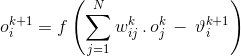
\includegraphics[scale=0.64]{neuronoutput}\end{center}
\caption[neuronoutput]{Výstupná hodnota neurónu~\cite{kvasnivcka1997uvod}}\label{fig:neuronoutput}
\end{figure}

%\newline
\noindent



\begin{figure}[H]
\begin{center}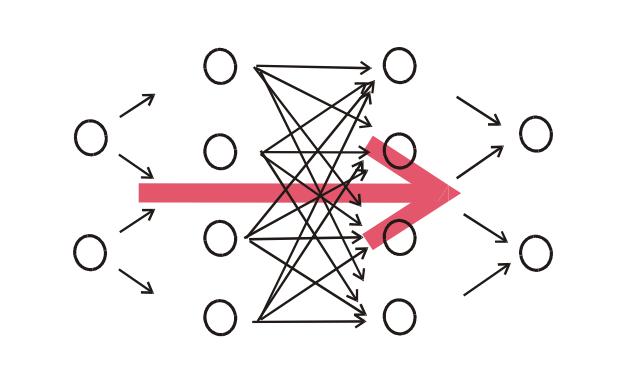
\includegraphics[scale=0.64]{fnn}\end{center}
\caption[fnn]{Štruktúra doprednej neurónovej siete (FNN)~\cite{jaeger2002tutorial}}\label{fig:fnn}
\end{figure}

\section{Učenie neurónovej siete}
\label{analyza_ucenie_nn}

Učenie predstavuje kľúčovú aktivitou pre schopnosť siete produkovať požadované výsledky. Spočíva vo vystavovaní neurónovej siete tréningovým dátam, ktoré sa sieť snaží interpretovať.

\textbf{Učenie s učiteľom} je metóda, pri ktorej je dostupná sada tréningových dát ,,označená". Pri interpretovaní výsledku je možné okamžite určiť, aká chyba nastala a následne ju propagovať do siete. Na toto sa využíva tzv. \textit{spätná propagácia}(backpropagation), ktorá upravuje váhy siete v rozsahu chyby, ktorá nastala - rozdiel medzi správnym výsledkom pre daný vstup a samotným výsledkom siete.
\noindent

\textbf{Učenie bez učiteľa} predstavuje alternatívnu metódu, pri ktorej tréningové dáta nemajú dostupné výsledky. Neurónová sieť sa sama učí rozhodnúť, čo je pre ňu relevantné. Učenie bez učiteľa predstavuje možnosť ako získať takmer neobmedzené množstvá tréningových dát tam, kde učenie s učiteľom vyžaduje manuálne a kvôli časovej náročnosti nedostupné označovanie.
\noindent

\section{Optimalizácia}
\label{optimalization}

Snahou optimalizácie je hľadať ideálne riešenie v často obrovskom prehľadávanom priestore. V prípade neurónových sietí je to hľadanie optimálneho nastavenia siete, ktorá následne dokáže meniť vstup na predpokladaný výstup. Asi najčastejšou úlohou optimalizačných techník v neurónových sieťach je minimalizovať stratu(angl. \textit{loss}). Tá naznačuje, ako ďaleko sa naša sieť nachádza od konvergencie k ideálnemu riešeniu. Je definovaná ako súčet chýb, ktoré boli dosiahnuté v tréningových alebo validačných množinách. Pri učení sa snažíme optimalizovať stratu, ale nie nulovať ju. V bežných prípadoch pri zašumených dátach totiž nulová chyba znamená preučenie - kopírovanie datasetu namiesto odhaľovania vzorov v ňom.

\subsection{Gradient descent}
\label{stochastic_gradient_descent}

Gradient descent predstavuje stratégiu spätnej propagácie v ktorej je vypočítaná derivácia chyby a tá je následne prenesená do parametrov siete ich upravovaním pre minimalizáciu chyby v nasledujúcej iterácii. 

Obľúbená varianta je \textbf{stochastický gradient descent}, ktorý je síce menej presný, ale prenáša chybu po každej iterácii, narozdiel od originálneho stochastického gradientu, ktorý upravuje parametre až po celej sade. Ajkeď teda SGD nedosiahne presnosť GD, dostane sa do blízkosti riešenia oveľa rýchlejšie a bude tam oscilovať. Táto vlastnosť ho uprednostňuje pri väčších datasetoch.

Pri používaní gradient descent algoritmu je problematické správne odhadnúť hyperparametre. Bežný postup je preskúmať široké okolie a sledovať ako vplýva zmena hyperparametrov na schopnosť minimalizácie chyby~\cite{zhang2004solving}.


\section{Hyperparametre}
\label{analyza_hyperparametre}

Nastavenia, pomocou ktorých kontrolujeme správanie neurónových sietí sa nazývajú \textit{hyperparametre}. Tieto hodnoty nie sú získané učením siete pokiaľ nemodelujeme vnorený systém za týmto účelom. Príkladom hyperparametra je počet skrytých vrstiev NN. Pri nízkom počte nebude model schopný naučiť sa funkciu definovanú problémom. Pri vysokom počte je možné, že sieť v sebe uloží menší tréningový dataset, nazývané tiež ako problém \textit{preučenia}(overfitting). Pri preučení sieť nezíska schopnosť generalizácie problému kvôli sledovaniu tréningového datasetu. Je zjavné, že zvolenie správnych hyperparametrov má pre výsledky metódy kľúčovú úlohu~\cite{Goodfellow-et-al-2016-Book}.
 Medzi ďaľšie významné hyperparametre patria:
\begin{my_itemize}
	\item {Šírka jednotlivých vrstiev} - ovplyvňuje koľko prepojení existuje a mení tak nároky siete na učenie ako aj zložitosť vzorov, ktoré sa sieť dokáže naučiť.
	\item {Rýchlosť učenia} - rozhoduje o tom, v ako rozsahu bude upravovaná sieť pri spätnej propagácií. Vystupuje ako kvantifikátor aplikovanej zmeny váh.
	\item {Momentum} - predstavuje riešenie pre problém lokálneho minima aj pre osciláciu pri stochastickom gradient descente. Vysoké momentum je schopné prekonať lokálne minimum a pri oscilácii okolo globálneho riešenia sa spomaľuje~\cite{attoh1999analysis}.
\end{my_itemize}

\section{Aktivačná funkcia}
\label{activation_function}

Aktivácia je matematická operácia aplikovaná na výstupy z predchádzajúcej vrstvy. Mení vstupné hodnoty na výstupný signál. 

\textbf{Sigmoidná funkcia} - Produkuje signál v kladnom rozsahu $<0,1>$. Najefektívnejšia je pre dáta ktoré sú na vstupe v rovnakom rozsahu~\cite{sibi2013analysis}.

\textbf{ReLU} - Usmernená lineárna jednotka, predstavuje najjednoduchšiu derivovateľnú nelineárnu funkciu. Nesaturuje výstup a vďaka tomu dosahuje dobré výsledky pre hlboké neurónové siete - nevzniká efekt miznúceho gradientu.
	
\textbf{Softmax} - Funkcia najčastejšie využívaná pri klasifikačných úlohách na výstupe. Škáluje výsledné neuróny tak, aby spoločný výstupný signál dosahoval hodnotu 1. ~\cite{toth2013phone}


\section{Rekurentné neurónové siete}
\label{analyza_pokrocile_modely_nn}

Do popredia výskumu sa v súčasnosti dostávajú pokročilé modely, ktoré už nie sú obmedzené na jednoduchý dopredný prístup. Vďaka rapídnemu zvyšovaniu výkonu grafických kariet sa čoraz častejšie aplikujú \textit{rekurentné modely neurónových sietí}(RNN)~\cite{jaeger2002tutorial}. Špecializáciou rekurentných sietí je práca so sekvenčnými dátami. Tieto siete predstavujú generalizáciu dopredných modelov ich rozšírením o cyklické prepojenia~\cite{Goodfellow-et-al-2016-Book}.
Takýmto spôsobom je možné využiť súčasnú hodnotu premennej na ovplyvnenie vlastnej hodnoty v budúcnosti. Cyklický charakter rekurentného modelu je zobrazený na obr.~\ref{fig:rnn}.

\begin{figure}[H]
\begin{center}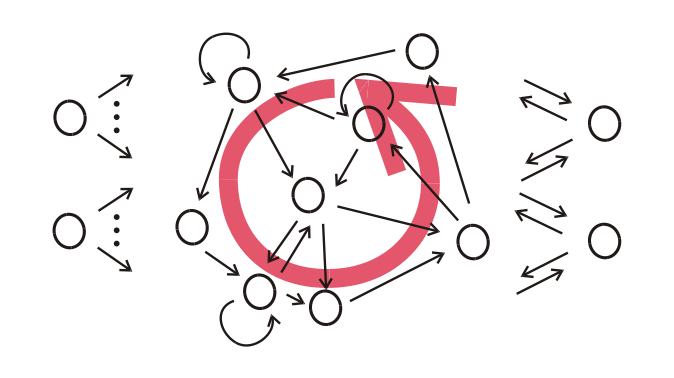
\includegraphics[scale=0.64]{rnn}\end{center}
\caption[rnn]{Štruktúra rekurentnej neurónovej siete~\cite{jaeger2002tutorial}}\label{fig:rnn}
\end{figure}

\section{Siete s dlhou krátkodobou pamäťou - LSTM}


LSTM predstavuje vylepšený model RNN. Vnútorná štruktúra ako doplnok ku externej rekurencii medzi jednotlivými neurónmi obsahuje aj \textit{internú rekurenciu}, zobrazenú v štruktúre LSTM neurónu na obr.~\ref{fig:lstm}. Medzi najdôležitejšie súčasti tohto modelu patria sigmoidné brány, ktoré rozhodujú o tom, ako sa signál bude širiť. LSTM tak prekonáva problém strácajúceho sa gradientu, ktorým trpí klasická RNN architektúra~\cite{hochreiter1997long}.
\newline
\textbf{Brána zabudnutia} ovplyvňuje, či nastáva vnútorná rekurencia neurónu. Stav tak môže ale nemusí byť faktorom ovplyvňujúcim nasledujúcu iteráciu výpočtu v sieti. Významné zlepšenie v LSTM sieťach prišlo s myšlienkou \textit{kontextom podmieneného zabúdania}. Takýto model sa ukazuje extrémne výhodným pri riešení problémov zahŕňajúcich \textit{časové pauzy}(lags)~\cite{gers2000learning}.
 Dôležitý prvok  na obr.~\ref{fig:lstm} predstavuje čierna kocka. Označuje pauzu o veľkosti jednej iterácie. Hodnota signálu tak ovplyvňuje nasledujúcu iteráciu, tj. vplýva na neskoršie udalosti.
\newline
\noindent


%ako do riti mam prelozit peepholes? 
\textbf{Nazeracie diery}(peepholes) predstavujú vylepšenie LSTM. Rieši problémy, ktoré vznikajú na základe faktu, že brána nedostáva priame informácie o stave jadra LSTM bloku(CEC). Táto situácia nastáva, keď je výstupná brána zatvorená. \textit{Nazeranie} predstavuje techniku váhovaného prepojenia CEC s bránami bloku daného jadra. Prepojenia sú štandardné s výnimkou časovej pauzy.

LSTM siete v praxi dokázali svoje schopnosti pri aplikácií na rôzne netriviálne dátové problémy. Pozornosť je kladená na frekventovanú časovú závislosť v dátach:
%deeplearning LSTM ma odkazy na konkretne projekty
\begin{my_itemize}
	\item{Rozoznávanie rukopisu} ~\cite{greff2015lstm}
	\item{Rozoznávanie reči} ~\cite{graves2013speech}
	\item{Označovanie obrázkov} ~\cite{kiros2014unifying}
\end{my_itemize}


\begin{figure}[H]
\begin{center}
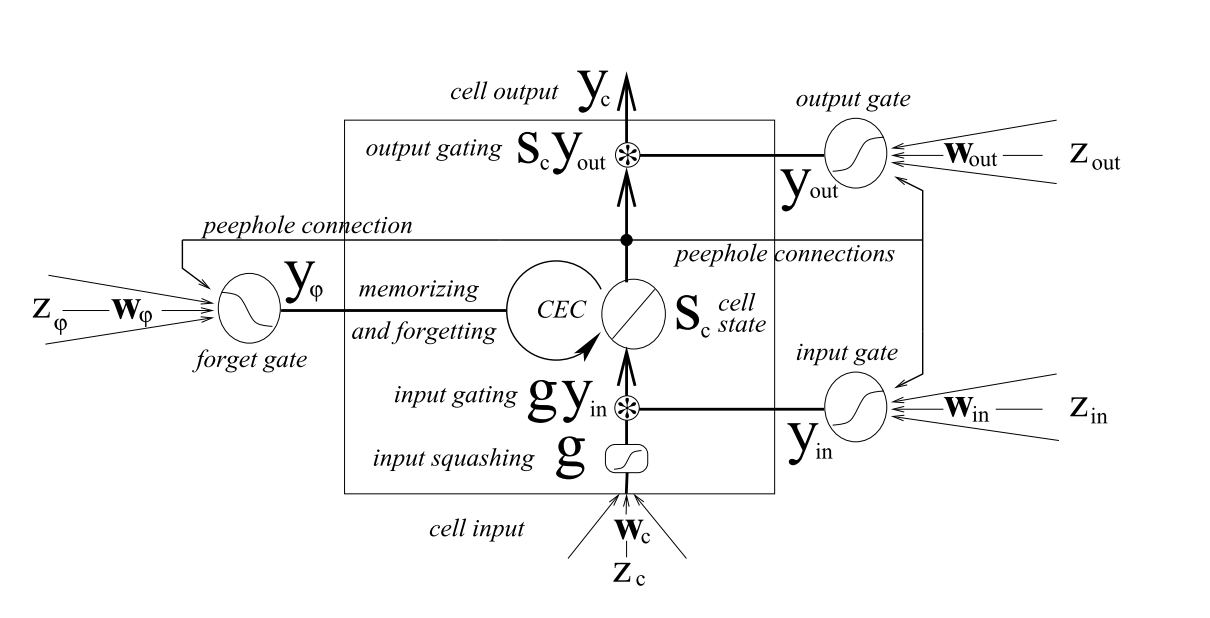
\includegraphics[scale=0.50]{peepholes}\end{center}
\caption[peepholes]{Schéma nazerania v LSTM bloku~\cite{gers2003learning}}
\label{fig:lstm}
\end{figure}

\chapter{Výskum v danej oblasti}
\label{analyza_vyskum_danej_oblasti}

V tejto časti sa zaoberáme štúdiami skúmajúcimi aplikáciu data-miningu pri generovaní odporúčaní a aplikáciou neurónových sietí v dátovej analytike. Tieto štúdie vedú k optimalizácii poskytovania online produktov a služieb.

\section{RecSys Challenge 2015}
\label{recsys_challenge}

RecSys Challenge 2015 bola súťaž v data-miningu zameranom na odporúčacie zariadenia vyhlásená organizáciou ACM. Súťažiaci mali možnosť implementovať riešenie, ktoré by dokázalo s čo najväčšou úspešnosťou predpovedať na testovacej množine nákupy v online obchode~\cite{ben2015recsys}.

\subsection{Dáta}
Pre túto súťaž boli poskytnuté dáta od vlastníka väčšieho európskeho portálu pre elektronický predaj. Dáta reprezentujú zhruba 6 mesačnú aktivitu používateľov na portáli. Dokopy súbory obsahujú vyše 33 miliónov záznamov z klikov zoskupených do 9.5 milióna sessions. Z toho bolo predaných 1.1 milióna položiek. Dáta sú rozdelené do dvoch súborov:

\begin{my_itemize}
	\item{yoochoose-clicks.dat}\newline
	- ID session, čas, ID položky, kategória položky
	\newline
	\item{yoochoose-buys.dat}\newline
	- ID session, čas, ID položky, cena, množstvo
	
\end{my_itemize}

Cieľom súťaže bolo predpovedať, ktoré používateľské sessions budú nákupné a ktoré z prehliadaných položiek budú kúpené. Metrikou pre úspešnosť bol vzorec:


\label{recsys_evaluation}
$$
score(Sl)=\Sigma_{\forall S \in Sl} =\\
\begin{cases}
	if s \in Sb \to \frac{Sb}{S} + \frac{|AS\cap BS|}{|AS\cup BS|} \\
	else \to -\frac{Sb}{S}\\
\end{cases}
$$

kde platí:

\begin{my_itemize}
	\item{Sl} - počet session vložených ako riešenie
	\item{S} - počet všetkých sessions v teste
	\item{s} - session v teste
	\item{Sb} - počet nákupných sessions v teste
	\item{As} - sada predikovaných nákupov v session s
	\item{Bs} - sada kúpených položiek v session s
\end{my_itemize}

Perfektné skóre dosiahnuteľné pre tento dataset s danou metrikou je 135176, pričom víťazný tím dosiahol skóre 63102. Na obrázku \ref{fig:recsys} možno sledovať najlepšie riešenia v priebehu mesiacov.

\begin{figure}[H]
	\begin{center}
		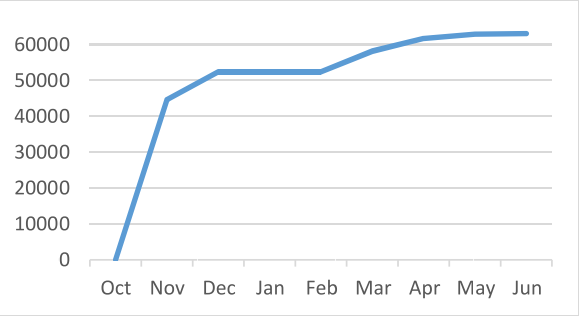
\includegraphics[scale=0.50]{recsys}\end{center}
	\caption[recsys]{Najlepšie priebežné výsledky počas trvania súťaže~\cite{ben2015recsys}}
	\label{fig:recsys}
\end{figure}


\subsection{Predikcia nákupov pomocou LSTM BiRNN}
\label{yoochoose_lstm}

Štúdia~\cite{wu2015neural} využíva rekurentnú neurónovú sieť s krátkou dlhodobou pamäťou(LSTM) pri predikcií YooChoose datasetu vzorov v klikaní na stránkach internetového predajného portálu. Prístup oddeľuje dve separátne problematiky - predikciu nákupných sessions a následne predikciu kúpených položiek. 

Dostupné dáta~\ref{recsys_challenge} sú predspracované na vstup do neurónovej siete. Tá následne po tréningu predpovedá výsledky pre testovacie dáta. Po predspracovaní vyzerajú jednotlivé vstupy do siete nasledovne:\newline
\linebreak


\parbox{.45\linewidth}{

	\begin{tabular}{||c||} 
		\hline
		Predpovedanie položiek  \\ [0.5ex] 
		\hline\hline
		Mesiac  \\ 
		\hline
		Deň v týždni  \\
		\hline
		Čas dňa(minúty) \\
		\hline
		Počet klikov na položku \\
		\hline
		Počet nákupov položky  \\ 
		\hline
		Aktuálna cena položky  \\
		\hline
		Maximálna cena položky \\
		\hline
		Minimálna cena položky \\
		\hline
		Položka na predaj \\
		\hline
		Trvanie kliku \\
		\hline
		Kategória \\ [1ex] 
		\hline
	\end{tabular}
}
\parbox{.45\linewidth}{
	\begin{tabular}{||c||} 
		\hline
		Predpovedanie nákupnej session  \\ [0.5ex] 
		\hline\hline
		Počet kikov v session  \\ 
		\hline
		Počet unikátnych položiek v session  \\
		\hline
		Počet klikov za minútu \\
		\hline
		Minimálny počet klikov v session \\
		\hline
		Maximálny počet klikov v session  \\ 
		\hline
		Priemerný počet klikov \\
		\hline
		Trvanie session \\
		\hline
		Priemerné trvanie kliku\\
		\hline
		Minimálna dĺžka kliku \\
		\hline
		Maximálna dĺžka kliku \\
		\hline
		... \\ [1ex] 
		\hline
	\end{tabular}
}

Táto práca sa porovnala s niekoľkými ďaľšími metódami ako gradient-boosting regresia a hlboká neurónová sieť (DNN). Skóre sa odvíja od metriky pre yoochoose dataset ~\ref{recsys_evaluation}.

\begin{figure}[H]
	\begin{center}
		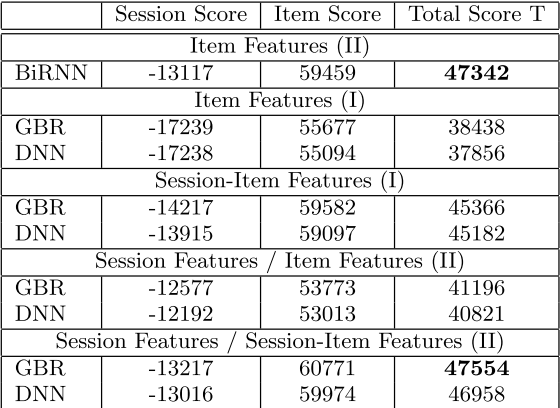
\includegraphics[scale=0.56]{recsys_yoochoose}\end{center}
	\caption[pixelmap]{Vyhodnotenie}
	\label{fig:evaluation}
\end{figure}


\subsection{Hlboká konvolučná neurónová sieť}
\label{metoda_konvolucna}


Pokročilé modely neurónových sietí ako hlboké konvolučné siete dosahujú veľmi dobré výsledky pri problémoch spracovania obrazu~\cite{szegedy2015going}.
Za účelom využitia týchto vlastností štúdia skladá z používateľskej aktivity obrazovú mapu - dvojrozmerné pole normalizovaných pixelov. Za účelom učenia má každý obraz dostupné označenie, ktoré hovorí či daný zákazník prešiel ku konkurencii alebo nie. Obr.~\ref{fig:pixelmap} zobrazuje ukážku aktivity zákazníka v dostupných službách za posledných $n$ dní~\cite{wangperawong2016churn}.

\begin{figure}[H]
\begin{center}
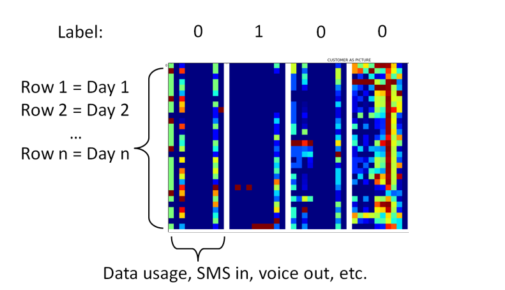
\includegraphics[scale=0.92]{pixelmap}\end{center}
\caption[pixelmap]{Aktivita zákazníka v mape pixelov. Hodnota pixelov sa zvyšuje od modrej k červenej
~\cite{wangperawong2016churn}.}
\label{fig:pixelmap}
\end{figure}

Experiment uvažuje 30-dňové okno predikcie, z ktorého sieť usudzuje aktivitu zákazníka. Okno sa nachádza 14 dní pred posledným registrovaný telefonátom. Pokiaľ sa posledný registrovaný telefonát nekonal v posledných 14 dňoch od aktuálneho dátumu, považujeme zákazníka za neaktívneho a neberieme ho do úvahy.
\newline
Po vytvorení obrazového datasetu z dostupných záznamov boli dáta podsunuté konvolučnej neurónovej sieti na obr.~\ref{fig:convolutional}.
Táto sieť má architektúru podobnú iným sieťam určeným pre spracovanie obrazu. Sieť analyzuje týždňové vzory v aktivite pomocou 7x1 filtra prvej konvolučnej vrstvy. Na konci siete je pomocou binárneho softmax klasifikátora vyhodnotený výsledok.
\newline

\begin{figure}[H]
\begin{center}
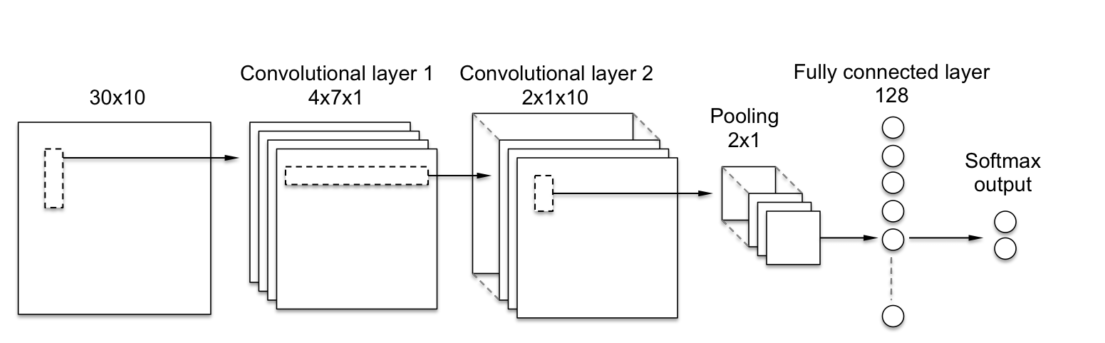
\includegraphics[scale=0.46]{convolutional}
\caption[convolutional]{Architektúra konvolučnej siete pre klasifikáciu zákazníkov z pixelovej mapy aktivity~\cite{wangperawong2016churn}.}
\label{fig:convolutional}
\end{center}
\end{figure}

Pomocou metódy \textit{oblasti pod krivkou}(AUC) bolo zistené, že konvolučná sieť dosahuje lepšie výsledku ako model CHAID rozhodovacieho stromu. AUC vyhodnocuje pravdivé aj nepravdivé pozitívne výsledky~\cite{hanley1982meaning}~\cite{bradley1997use}.

